\documentclass[12pt]{article}
\usepackage{amsmath,amsthm,amssymb}
\usepackage{geometry}
\usepackage{makeidx}
\usepackage{graphicx}
\usepackage{color}
\usepackage[usenames,dvipsnames]{xcolor}
\usepackage{tikz}
\usetikzlibrary{calc}
\usepackage{xfrac}
\usepackage{array}
\usepackage{color}
\usepackage{listings}
\usepackage{bbm}
\lstset{ %
language=C++,
basicstyle=\footnotesize,
numbers=left,
numberstyle=\footnotesize,
stepnumber=1,
numbersep=5pt,
backgroundcolor=\color{white},
showspaces=false,% show spaces adding particular underscores
showstringspaces=false,% underline spaces within strings
showtabs=false,% show tabs within strings adding particular underscores
tabsize=2,% sets default tabsize to 2 spaces
captionpos=b,% sets the caption-position to bottom
breaklines=true,% sets automatic line breaking
breakatwhitespace=false,
escapeinside={\%*}{*)}          % if you want to add a comment within your code
}
\usepackage{xstring}

\usepackage[english,greek]{babel}
\usepackage[utf8x]{inputenc}
%\usepackage{ucs}

\usepackage{enumerate}
\usepackage{enumitem}
\setlist{nolistsep}
\usepackage{hyperref}
\hypersetup{colorlinks=true,linkcolor=MidnightBlue}

\newcommand\en[1]{\latintext #1\greektext}
\newcommand\m[1]{\mbox{$\displaystyle #1 $}}
\newcommand\ul[1]{\emph{#1}}
\newcommand\bigOh{\mathcal{O}}
\newcommand\nospace{\hspace*{-0.5em}}

\renewcommand{\thefootnote}{*}

\newenvironment{n_enum}{
\begin{enumerate}[label=(\arabic{*})]
  \setlength{\itemsep}{0pt}
  \setlength{\parskip}{0pt}
  \setlength{\parsep}{0pt}
}{\end{enumerate}}

\newenvironment{i_enum}{
\begin{enumerate}[label=(\roman{*})]
  \setlength{\itemsep}{0pt}
  \setlength{\parskip}{0pt}
  \setlength{\parsep}{0pt}
}{\end{enumerate}}

\newenvironment{a_enum}{
\begin{enumerate}[label=(\alph{*})]
  \setlength{\itemsep}{0pt}
  \setlength{\parskip}{0pt}
  \setlength{\parsep}{0pt}
}{\end{enumerate}}

\newenvironment{b_item}{
\begin{itemize}
  \setlength{\itemsep}{0pt}
  \setlength{\parskip}{0pt}
  \setlength{\parsep}{0pt}
}{\end{itemize}}

\newcommand{\HRule}{\rule{\linewidth}{0.1mm}}

\begin{document}
\begin{center}
{\bf Αλγόριθμοι και πολυπλοκότητα}\\
3η Σειρά Γραπτών ασκήσεων
\end{center}
Χειμερινό Εξάμηνο 2013-2014 \hfill Μπογιόκας Δημήτριος - ΜΠΛΑ
\HRule\\
{\bf Άσκηση 1} Ένας γραμμικός αλγόριθμος που υπολογίζει το πλήθος των διαφορετικών $s-v$ μονοπατιών για κάθε κορυφή $v\in V\setminus\{s\}$ ενός κατευθυνόμενου γραφήματος $G(V,E)$ με μοναδιαία μήκη ακμών, βασίζεται στον αλγόριθμο \en{bfs}. Συγκεκριμένα, αρχικοποιώ έναν πίνακα \en{amount(v)} στο 0 για κάθε $v\in V\setminus\{s\}$ και \en{amount(s)=1} που για κάθε κορυφή $v$ θα μετράει το ζητούμενο πλήθος. Ο αλγόριθμος θα κάνει αναζήτηση \en{bfs} στο γράφημα. Για κάθε ακμή $(u,v)$, θα εξετάζει αν η κορυφή $v$ βρίσκεται σε απόσταση \en{dist(u)+1} και σε αυτή την περίπτωση θα θέτει \en{amount(v)+=amount(u)}, δηλαδή θα αυξάνει το πλήθος των μονοπατιών που καταλήγουν στην υπό εξέταση κορυφή $v$ κατά το πλήθος των μονοπατιών που φτάνουν στην εξερευνημένη κορυφή $u$. Ο αλγόριθμος γραμμένος σε ψευδοκώδικα είναι:
\latintext\begin{lstlisting}
int* bfs_amount(G,s) {
  //Input:  Directed Graph G=(V,E) and vertex s in V.
  //Output: List amount(v), which is set to be the amount of the distinct s-v paths of minimum lenght.

  forall u in V {
    dist(u)=infty;
  }
  dist(s)=0;

  forall u in V {
    amount(u)=0;
  }
  amount(s)=1;

  Q=[s]; //queue of bfs
  while Q notempty {
    u=eject(Q);
    forall (u,v) in E {
      if dist(v)==infty {
        inject(Q,v);
        dist(v)=dist(u)+1;
      }
      if dist(v)==dist(u)+1 {
        amount(v)+=amount(u);
      }
    }
  }

  return amount;
}
\end{lstlisting}\greektext
Η ορθότητα του αλγορίθμου αποδεικνύεται επαγωγικά. Θέτω
$$a\left(s,v\right):=\#\left\{P\left(s,v\right):|P\left(s,v\right)|=d\left(s,v\right)\right\}$$
όπου $P\left(s,v\right)$ κάποιο μονοπάτι από το $s$ στο $v$ και $d\left(s,v\right)$ η απόσταση από το $s$ στο $v$.
Τότε ισχύει προφανώς το εξής:
$$a\left(s,v\right)=\sum_{\underset{d\left(s,u\right)=d\left(s,v\right)-1}{\underset{(u,v)\in E}{u\in V}}}a\left(s,u\right)$$
το οποίο είναι ακριβώς αυτό που υπολογίζει αναδρομικά και ο παραπάνω αλγόριθμος. Για τη βάση της επαγωγής, το πλήθος των μονοπατιών από το $s$ στο $s$ είναι ακριβώς $1$, με τετριμμένο τρόπο. Ο αλγόριθμος τρέχει σε γραμμικό χρόνο $\bigOh(n+m)$, καθώς εξετάζει κάθε ακμή ακριβώς μία φορά, όπως ακριβώς και ο \en{bfs}. Ο αλγόριθμος γενικεύεται ως εξής: Σε γραμμικό χρόνο, ελέγχοντας μία φορά κάθε ακμή κατασκευάζω γράφημα $G'$ όπου προκύπτει με υποδιαίρεση κάθε ακμής του $G$, βάρους $l\in\left\{1,\ldots,k\right\}$ σε ένα μονοπάτι με $l$ ακμές μοναδιαίου βάρους. Στη συνέχεια εφαρμόζω τον παραπάνω αλγόριθμο στο $G'$. Το $G'$ έχει $(k-1)m+n$ κορυφές και $km$ ακμές, άρα ο αλγόριθμος κάνει χρόνο $\bigOh((k-1)m+n+km)=\bigOh(n+m)$ αφού το $k$ θεωρείται σταθερό. (ουσιαστικά πρόκειται για μια απλοποίηση του αλγορίθμου του \en{Dijkstra}).\\
\HRule\\
{\bf Άσκηση 2} Εφ' όσων το $G$ είναι κατευθυνόμενο ακυκλικό γράφημα, υπάρχει τουλάχιστον μία κορυφή του $v\in V$ που έχει \en{indegree} μηδέν. Σε γραμμικό χρόνο υπολογίζω το \en{indegree} όλων των κορυφών (ελέγχω κάθε ακμή μία φορά). Εάν υπάρχουν πάνω από μία κορυφές με \en{indegree} ίσο με μηδέν, τότε δεν υπάρχει μονοπάτι \en{Hamilton}, διαφορετικά, υπάρχει μοναδική πηγή, έστω $s$. Αφαιρούμε την $s$ από το γράφημα, μειώνοντας τον \en{indegree} κάθε κορυφής $u$ με $(u,v)\in E$ κατά ένα και ελέγχοντας ταυτόχρονα πόσες από αυτές κατέληξαν με \en{indegree} μηδεν. Καθώς ένα γράφημα παραμένει ακυκλικό, αφαιρόντας του μία κορυφή, θα υπάρχει τουλάχιστον ένας γείτονας που θα είναι πλέον πηγή. Αν υπάρχουν περισσότεροι του ενός, δεν υπάρχει μονοπάτι \en{Hamilton}. Εάν υπάρχει μοναδικός γείτονας, ο αλγόριθμος συνεχίζει επαγωγικά μέχρι να εξαντληθούν οι κορυφές ή μέχρι να βρεθεί πιστοποιητικό μη ύπαρξης μονοπατιού \en{Hamilton}. Ο αλγόριθμος σε ψευδοκώδικα είναι:
\latintext\begin{lstlisting}
Hamilton_path(G,s) {
  //Input:  Directed Graph G=(V,E).
  //Output: prints the nodes in the order of the Hamilton path, until all nodes are printed or until it prints which two nodes have indegree 0.

  forall u in V {
    indegree(u)=0;
  }

  forall (u,v) in E {
    indegree(v)++;
  }

  foundfirstsource = false;
  existsHamilton = true;

  node source;
  node secondsource;

  forall u in V' {
    if indegree(u)==0 {
      if foundfirstsource {
        existsHamilton = false;
        secondsource = u;
        break;
      }
      else {
        foundfirstsource = true;
        source = u;
      }
    }
  }

  if !existsHamilton {
    print "There exists no Hamilton path, because " source " and " secondsource " have both outdegree 0 in the Graph";
    return;
  }

  print source;

  V' = V-{source};

  while V' notempty {
    foundfirstsource = false;
    existsHamilton = true;

    node newsource;
    node secondsource;

    forall u in N(source) { //Neighbourhood of source
      indegree(u)--;
      if indegree(u)==0 {
        if foundfirstsource {
          existsHamilton = false;
          secondsource = u;
          break;
        }
        else {
          foundfirstsource = true;
          newsource = u;
        }
      }
    }

    if !existsHamilton {
      print "There exists no Hamilton path, because " newsource " and " secondsource " have both outdegree 0 in the remaining Graph";
      return;
    }
    source = newsource;
    print source;
    V'=V'-{source};
  }
  return;
}
\end{lstlisting}\greektext
Η ορθότητα του αλγορίθμου βασίζεται στο γεγονός ότι αν ένα \en{DAG} έχει \en{Hamilton path}, τότε αυτό αρχίζει από μία πηγή και δεν ξαναπερνάει ποτέ από πηγή, άρα ένα γράφημα με δύο πηγές δεν έχει \en{Hamilton path}. Ο αλγόριθμος τρέχει σε γραμμικό χρόνο, καθώς αρχικά χρειάζεται $\bigOh(n+m)$ για να αρχικοποιήσει τον πίνακα \en{indegree} και στη συνέχεια $\bigOh(m)$, γιατί στη συνέχεια εξετάζει κάθε ακμή μία ακριβώς φορά.\\
\HRule\\
{\bf Άσκηση 3} Ένας αλγόριθμος που λύνει το πρόβλημα σε χρόνο $\bigOh(m\log\log n)$ είναι συνδυασμός των αλγορίθθμων του \en{Prim} και του \en{Bor\.uvka}. Ο αλγόριθμος του \en{Bor\.uvka} είναι ο εξής:\\
Για κάθε κορυφή $v\in V$ του γραφήματος, ο αλγόριθμος επιλέγει την ακμή ελαχίστου βάρους, έστω $e_v$ που προσπίπτει στην κορυφή $v$. Με αυτό τον τρόπο πράγματι επιλέγονται ακμές που ανήκουν τελικά σε κάποιο \en{spanning tree} ελαχίστου βάρους, καθώς κάθε μία από αυτές είναι η ελάχιστη που συνδέει τα σύνολα $\{v\},V\setminus\{v\}$ στο αρχικό γράφημα. Για να επιλέξει αυτές τις $|V|$ ακμές χρειάζεται χρόνο $\bigOh(2|E|)$. Πράγματι, για κάθε κορυφή βαθμού $d_v$ βρίσκει την προσπίπτουσα ακμή ελαχίστου βάρους σε χρόνο $\bigOh(d_v)$, δηλαδή συνολικά ο αλγόριθμος χρειάζεται χρόνο
$$\bigOh\left(\sum_{v\in V}d_v\right)=\bigOh(2|E|)$$
Στη συνέχεια ο αλγόριθμος κατασκευάζει γράφημα $G'=(V',E')$ όπου κάθε κορυφή στο $V'$ αντιστοιχεί σε μία συνεκτική συνιστώσα του γραφήματος $G\left[\left\{e_v:v\in V\right\}\right]$ (συνεκτική συνιστώσα του γραφήματος που παράγεται από τις επιλεχθείσες ακμές). Για κάθε δύο κορυφές $u',v'\in V'$, η ακμή $\{u',v'\}$ υπάρχει στο καινούριο γράφημα (ανήκει στο $E'$), ανν υπάρχει ακμή στο αρχικό γράφημα που να συνδέει τις αντίστοιχες συνεκτικές συνιστώσες. Αν η ακμή υπάρχει στο καινούριο γράφημα, της ανατίθεται βάρος το ελάχιστο από τα βάρη των ακμών που συνδέουν τις δύο αυτές συνεκτικές συνιστώσες στο αρχικό γράφημα. Ταυτόχρονα για κάθε ακμή του καινούριου γραφήματος αποθηκεύει ο αλγόριθμος έναν δείκτη $\{u',v'\}.p$ που δείχνει στην αρχική ακμή με το ίδιο βάρος, ώστε να μπορεί αργότερα να ανακτηθεί. Στη συνέχεια ο αλγόριθμος κα\-λεί\-ται επαγωγικά με είσοδο $G'$, σε χρόνο $\bigOh(|E'|)=\bigOh(|E|)$ παράγοντας κάθε φορά ένα γράφημα με τις μισές κορυφές από το γράφημα της εισόδου και προσθέτοντας την ακμή $\{u',v'\}.p$ στο δέντρο, για κάθε ακμή $\{u',v'\}$ που επιλέγει. Ο αλγόριθμος του \en{Bor\.uvka} χρειάζεται χρόνο $\bigOh(m)$ σε κάθε επανάληψη, δηλαδή συνολικά χρόνο $\bigOh(km)$ μετά τις $k$ πρώτες επαναλήψεις. Εάν ο αλγόριθμος επαναληφθεί μέχρι να μείνει μία κορυφή (οι επιλεχθείσες ακμές να σχηματίσουν ένα \en{spanning tree}), τότε χρειάζεται $k=\bigOh(\log n)$ επαναλήψεις, αφού σε κάθε επανάληψη υποδιπλασιάζονται οι κορυφές. Από μόνος του αυτός ο αλγόριθμος δεν λύνει το πρόβλημα στον ζητούμενο χρόνο, αλλά επιλέγοντας το $k$ κατάλληλα και στη συνέχεια εφαρμόζοντας τον αλγόριθμο του \en{Prim} στο γράφημα με $n'=\frac{n}{2^k}$ κορυφές που προκύπτει μπορεί να βελτιωθεί το φράγμα. Πράγματι, ο αλγόριθμος του \en{Prim} μπορεί να υλοποιηθεί σε χρόνο $\bigOh(m'+n'\log n')$, χρησιμοποιώντας \en{Fibonacci heap}. Συνολικά δηλαδή, ο συνδυασμός των αλγορίθμων θα χρειαστεί χρόνο $\bigOh\left(mk+m+\frac{n}{2^k}\log\frac{n}{2^k}\right)$. Για $k=\bigOh(\log\log n)$ η παραπάνω ποσότητα ελαχιστοποιείται και γίνεται:
$$\begin{array}{rcl}\bigOh\left(m\log\log n+m+\frac{n}{\log n}\log\frac{n}{\log n}\right)
&=&\bigOh\left(m\log\log n+m+n-\log\log n\right)\\
&=&\bigOh\left(m\log\log n\right)\\
\end{array}$$
που είναι ακριβώς το ζητούμενο.\\
\HRule\\
{\bf Άσκηση 4}(α) Έστω $e=\{u,v\}$. Έστω $S,V\setminus S$ oποιαδήποτε διαμέριση κορυφών του γραφήματος σε δύο σύνολα, που διαχωρίζει τις κορυφές $u,v$. Το σύνολο
$$\left\{(v_1,v_2)\in E:v_1\in S,v_2\in V\setminus S\right\}$$
περιέχει την $e$ και τουλάχιστον άλλη μία ακμή του κύκλου $C$. Πράγματι, εάν όλες οι ακμές του κύκλου περιέχονταν στο ίδιο υποσύνολο της διαμέρισης, τότε το ίδιο θα ίσχυε και για τις κορυφές $u,v$, το οποίο είναι άτοπο. Άρα για κάθε τομή του γραφήματος, τέτοια ώστε η $e$ να ανήκει στο σύνολο τομής, υπάρχει κάποια άλλη ακμή στο σύνολο τομής (συγκεκριμένα τουλάχιστον μία ακόμη ακμή του $C$) που έχει το πολύ το ίδιο βάρος με την $e$, άρα, σύμφωνα με το άπληστο κριτήριο, η ακμή $e$ μπορεί να μην επιλεγεί για την κατασκευή κάποιου ελάχιστου συνδετικού δέντρου. Μαλιστα αν υπάρχει κάποια ακμή του συνόλου τομής με γνήσια μικρότερο βάρος, για κάθε τομή, τότε η $e$ σίγουρα δεν επιλέγεται.\\
\HRule\\
{\bf Άσκηση 4}(β) Εάν από ένα συνεκτικό γράφημα αφαιρεθεί κάποια ακμή που ανήκει σε κύκλο του γραφήματος, τότε το γράφημα παραμένει συνεκτικό. Άρα, δεδομένου ότι το αρχικό γράφημα είναι συνεκτικό, η ιδιότητα αυτή διατηρείται μέχρι και τον τερματισμό του αλγορίθμου. Επίσης, το γράφημα που προκύπτει τελικά είναι ακυκλικό. Πράγματι, έστω ότι υπάρχει κάποιος κύκλος στο τελικό γράφημα και έστω $e$ μια κορυφή μέγιστου βάρους του κύκλου αυτού. Τότε, καθώς με τη διαγραφή ακμών δε δημιουργούνται νέοι κύκλοι, ο κύκλος αυτός υπήρχε και στο αρχικό γράφημα, άρα εξετάζοντας ο αλγόριθμος την ακμή $e$, τη διαγράφει, άρα δε μένει στο τελικό γράφημα, άτοπο. Από αυτά τα δύο έπεται άμεσα ότι ο αλγόριθμος υπολογίζει ένα συνδετικό δέντρο. Η απόδειξη ότι το συνδετικό δέντρο που υπολογίζει ο αλγόριθμος είναι ελαχίστου βάρους γίνεται με επαγωγή στο $k$, όπου $k=|E|-|V|$. Πράγματι, αν για ένα γράφημα ισχύει ότι $k=|E|-|V|$, τότε αυτό περιέχει ακριβώς $k+1$ κύκλους. Για $k=0$, το γράφημα έχει έναν κύκλο $C$. Προφανώς, σε αυτή την περίπτωση κάθε ελάχιστο συνδετικό του δέντρο περιλαμβάνει όλες τις ακμές του γραφήματος εκτός από μία ακμή του κύκλου. Ο παραπάνω αλγόριθμος θα αφαιρέσει από το γράφημα την ακμή του $C$ που έχει μέγιστο βαρος, άρα σίγουρα το συνδετικό δέντρο που παράγει είναι ελαχίστου βάρους. Έστω ότι το ζητούμενο ισχύει για κάποιο $k\in\mathbb{N}$ και έστω ένα γράφημα $G$ τέτοιο ώστε $|E|=|V|+k+1$. Έστω επίσης $e$ η πρώτη ακμή που θα αφαιρέσει ο παραπάνω αλγόριθμος από το $G$. Για το γράφημα $G\setminus e$ ισχύει το ζητούμενο, αφού έχει μία ακμή λιγότερη (δηλαδή έναν κύκλο λιγότερο). Ο αλγόριθμος λοιπόν με είσοδο το $G\setminus e$ βρίσκει ένα ελάχιστο συνδετικό δέντρο του $G\setminus e$, έστω $T$. Από το (α), το $T$ είναι ένα ελάχιστο συνδετικό δέντρο του $G$. Αν ο αλγόριθμος τρέξει με είσοδο το $G$, θα αφαιρέσει αρχικά την ακμή $e$ και στη συνέχεια θα κάνει ακριβώς τα ίδια βήματα όπως θα έκανε αν έτρεχε με είσοδο το $G\setminus e$, άρα θα παράξει το συνδετικό δέντρο $T$, το οποίο απέδειξα όμως ότι είναι ελάχιστο, άρα από επαγωγή, ο αλγόριθμος υπολογίζει πάντα ένα ελάχιστο συνδετικό δέντρο.\\
\HRule\\
{\bf Άσκηση 4}(γ) Ένας γραμμικός αλγόριθμος που υπολογίζει ένα ελάχιστο συνδετικό δέντρο του $G$ κάνει $k+1$ επαναλήψεις του αλγορίθμου \en{dfs} στο $G$. Κάθε επανάληψη εκτελεί αναζήτηση \en{dfs} στο $G$ μέχρι να βρεθεί μια ακμή $\{u,v\}$ που ενώνει μια υπό εξέταση κορυφή $u$ με μια επίσης υπό εξέταση κορυφή $v$ (που είχε προηγηθεί στον αλγόριθμο από τη $u$). Στη συνέχεια, αρχίζοντας από την $u$ και ακολουθόντας τους δείκτες προς τον πρόγονο κάθε κορυφής στο \en{dfs} δέντρο που σχηματίστηκε, ο αλγόριθμος καταλήγει σε γραμμικό χρόνο στην $v$, εντοπίζοντας ακριβώς έναν κύκλο. Στη συνέχεια αφαιρεί την ακμή μέγιστου βάρους αυτού του κύκλου και σταματάει την επανάληψη. Καθώς το $k$ θεωρείται σταθερό, ο αλγόριθμος χρειάζεται συνολικά γραμμικό χρόνο. Ο αλγόριθμος εγγυάται την εύρεση ελάχιστου συνδετικού δέντρου, λόγω του ερωτηματος (α) (εφαρμοσμένου $k+1$ φορές).\\
\HRule\\
{\bf Άσκηση 5}(α) Ένα αντιπαράδειγμα γι αυτόν τον ισχυρισμό είναι το εξής:
\begin{center}
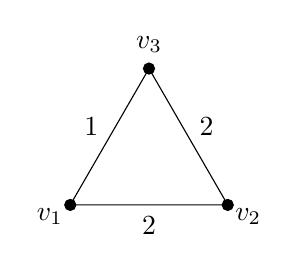
\begin{tikzpicture}
\foreach\x in {(0,0),(2,0),(60:2)}
 \filldraw[black] \x circle (2pt);
\draw (0,0)--(2,0)--(60:2)--(0,0);
\node at (210:0.3) {\m{v_1}};
\node at ($(2,0)+(-30:0.3)$) {\m{v_2}};
\node at ($(60:2)+(0,0.3)$) {\m{v_3}};
\node at (30:2) {\m{2}};
\node at ($(60:2)+(0,-2)$) {\m{2}};
\node at ($(2,0)+(150:2)$) {\m{1}};
\end{tikzpicture}
\end{center}
Στο παραπάνω γράφημα, το συνδετικό δέντρο που αποτελείται από τις ακμές $\{v_1,v_2\}$ και $\{v_2,v_3\}$ έχει βάρος $4$ και κάθε του ακμή περιέχεται σε κάποιο ελάχιστο συνδετικό δέντρο. Παρ' όλα αυτά κάθε ελάχιστο συνδετικό δέντρο του γραφήματος έχει βάρος $3$.\\
\HRule\\
{\bf Άσκηση 5}(β) Από τον ορισμό έπεται ότι μία ακμή $e$ είναι απαραίτητη για το Ελάχιστο Συνδετικό Δέντρο αν και μόνον αν περιέχεται σε κάθε Ελάχιστο Συνδετικό Δέντρο. Πράγματι, εάν υπήρχε κάποιο ελάχιστο συνδετικό δέντρο που δεν περιείχε την $e$, τότε αυτό θα ήταν συνδετικό δέντρο και στο γράφημα $G\setminus e$, άρα $MST(G\setminus e)\leq MST(G)$. Επίσης, εάν κάθε ελάχιστο δέντρο περιέχει την $e$, τότε κάθε ελάχιστο συνδετικό δέντρο του γραφήματος $G\setminus e$ θα έχει σίγουρα μεγαλύτερο βάρος από $MST(G)$, διότι διαφορετικά αυτό θα ήταν και ελάχιστο συνδετικό δέντρο του $G$.\\
\begin{i_enum}
\item Έστω ακμή $e$, για την οποία υπάρχει τομή τέτοια ώστε η $e$ να είναι η μοναδική ακμή ελαχίστου βάρους που την διασχίζει. Από την άπληστη επιλογή κατασκευής ενός οποιουδήποτε ελάχιστου συνδετικού δέντρου πρέπει η $e$ να επιλεχθεί στην κατασκευή του δέντρου, άρα είναι απαραίτητη ακμή. Αντίστροφα, έστω κάποια ακμή $e$ για την οποία ισχύει ότι για κάθε τομή που διασχίζει υπάρχει κάποια ακμή $e'$ η οποία είναι και αυτή ελαχίστου βάρους. Τότε, υπάρχει ελάχιστο συνδετικό δέντρο, όπου κατασκευάζεται αν σε κάθε μία από αυτές τις τομές επιλέγεται η $e'$ έναντι της $e$. Άρα τελικά κατασκευάζεται ελάχιστο συνδετικό δέντρο που δεν περιέχει την $e$, άρα δεν είναι απαραίτητη ακμή.
\item Έστω ότι για κάθε κύκλο, υπάρχει κάποια ακμή με μεγαλύτερο βάρος από την $e$ και ένα ελάχιστο συνδετικό δέντρο που δεν περιέχει την $e$, τότε προσθέτοντας την $e$ δημιουργείται ένας κύκλος, από τον οποίο αφαιρόντας την ακμή μεγαλύτερου βάρους από την $e$ θα προκύψει ένα συνδετικό δέντρο ακόμη μικρότερου βάρους, άτοπο. Άρα κάθε ελάχιστο συνδετικό δέντρο περιέχει την $e$. Αντίστροφα, εάν η ακμή $e$ ήταν ακμή μεγίστου βάρους για κάποιον κύκλο $C$, τότε από το 4(α), θα υπήρχε ελάχιστο συνδετικό δέντρο που δεν περιέχει την $e$, δηλαδή η $e$ δε θα ήταν απαραίτητη ακμή.
\end{i_enum}
\HRule\\
{\bf Άσκηση 5}(γ) Έστω ακμή $e=\{u,v\}\in E$. Ένας γραμμικός αλγόριθμος που αποφασίζει κατά πόσον η $e$ είναι απαραίτητη ακμή είναι ο ακόλουθος. Έστω $G'=G\setminus\left\{e'\in E\setminus\{e\}:w(e')\geq w(e)\right\}/e$ (όπου με $G/e$ συμβολίζω τη σύνθλιψη της ακμής $e$ μέσα στο γράφημα $G$). Έστω $w$ η κορυφή που προκύπτει από τη σύνθλιψη της $e$. Εφαρμόζω αλγόριθμο \en{dfs} στο $G'$, αρχίζοντας από την κορυφή $w$. Αυτό γίνεται σε γραμμικό χρόνο, κάνοντας \en{dfs} στο $G$, χωρίς να λαμβάνονται υπ' όψιν οι ακμές με βάρος $\geq w(e)$. Εάν κατά τη διάρκεια του \en{dfs} βρεθεί ακμή που να επιστρέφει στο $w$, τότε η $e$ δεν είναι απαραίτητη. Διαφορετικά, εάν ο \en{dfs} δεν βρει τέτοια ακμή (δεν υπάρχει κύκλος δηλαδή που να περιέχει την $e$ με τις υπόλοιπες ακμές γνήσια μικρότερου βάρους), τότε η $e$ είναι απαραίτητη ακμή. Η ορθότητα του αλγορίθμου έπεται άμεσα από τον δεύτερο χαρακτηρισμό του ερωτήματος (β).\\
\HRule\\
{\bf Άσκηση 5}(δ) Ένας αποδοτικός αλγόριθμος κάνει χρόνο $\bigOh(mn)$. Αρχικά χρησιμοποιόντας τον αλγόριθμο του \en{Prim} εντοπίζει ένα ελάχιστο συνδετικό δέντρο. Κάθε ακμή που δεν είναι στο συνδετικό δέντρο δεν είναι απαραίτητη ακμή, ενώ για κάθε μία από τις $n-1$ ακμές του ελάχιστου αυτού συνδετικού δέντρου, σε γραμμικό χρόνο ο αλγόριθμος εξετάζει κατά πόσον είναι όντως απαραίτητες ακμές, χρησιμοποιόντας τον αλγόριθμο του (γ). Συνολικά, ο αλγόριθμος χρειάζεται χρόνο $\bigOh(mlogm+(n+1)(m+n))=\bigOh(mn)$.
\end{document}
